\subsection{29 августа. Д.р. Кубань}
\textit{Метеоусловия: утром, днём ясно, жарко. Вечером~-- переменная облачность}

\begin{figure}[h!]
	\centering
	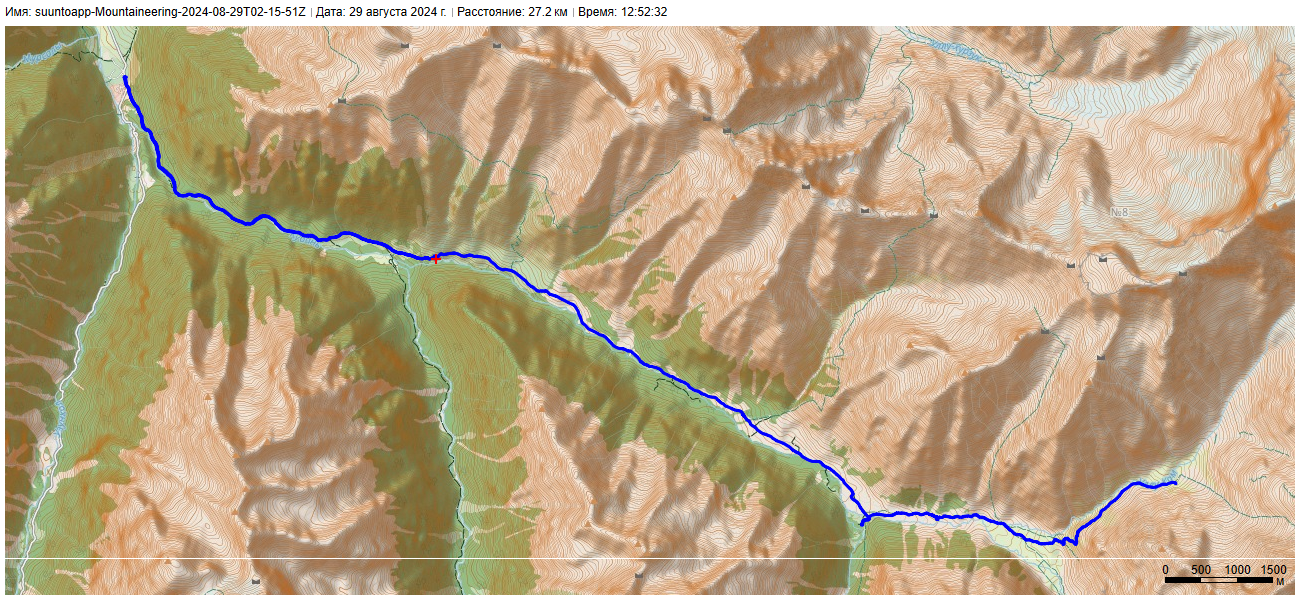
\includegraphics[angle=0, width=0.7\linewidth]{../pics/mini_maps/29}
	\label{fig:mini_29}
\end{figure}

*воспоминания вики: руководы отвели 4-х человек на трансфер, потом мы шли по пеклу, потом через кучу коровок и погранцов и еще одну кучу коровок, вверх по склону, красивый закатный траверс, стоянка среди камней*


Часть группы сходит с маршрута, вместе с руководителями встают в 4(?) и уходят в …, где их заберет трансфер. Для остальных подъем в 7, солнечно. Готовим завтрак, ждем возвращения руководителей, завтракаем, собираемся, выходим в 10 (?). Замечаем по ходу движения синие отметки на дороге, как позже оказалось, это разметка трейлраннингового маршрута.
Дорога в долине р. Кубань хорошая грунтовая, идет по открытой местности, иногда сменяется лесом. Жарко, у ручьев делаем привалы и набираем воду.

Подходим к загону для коров и постройкам местных жителей, преграждающих трек, обходим справа.
Переходим Кичкинекол (?) по мосту, чтобы отметиться у пограничников. На заставе никого нет, ждем 10 мин, уходим.
Продолжаем путь по грунтовой дороге, на карте в 500 м от дороги отмечен родник, идем азимутом по болотистой почве, родник не находим.

\begin{figure}[h!]
	\centering
	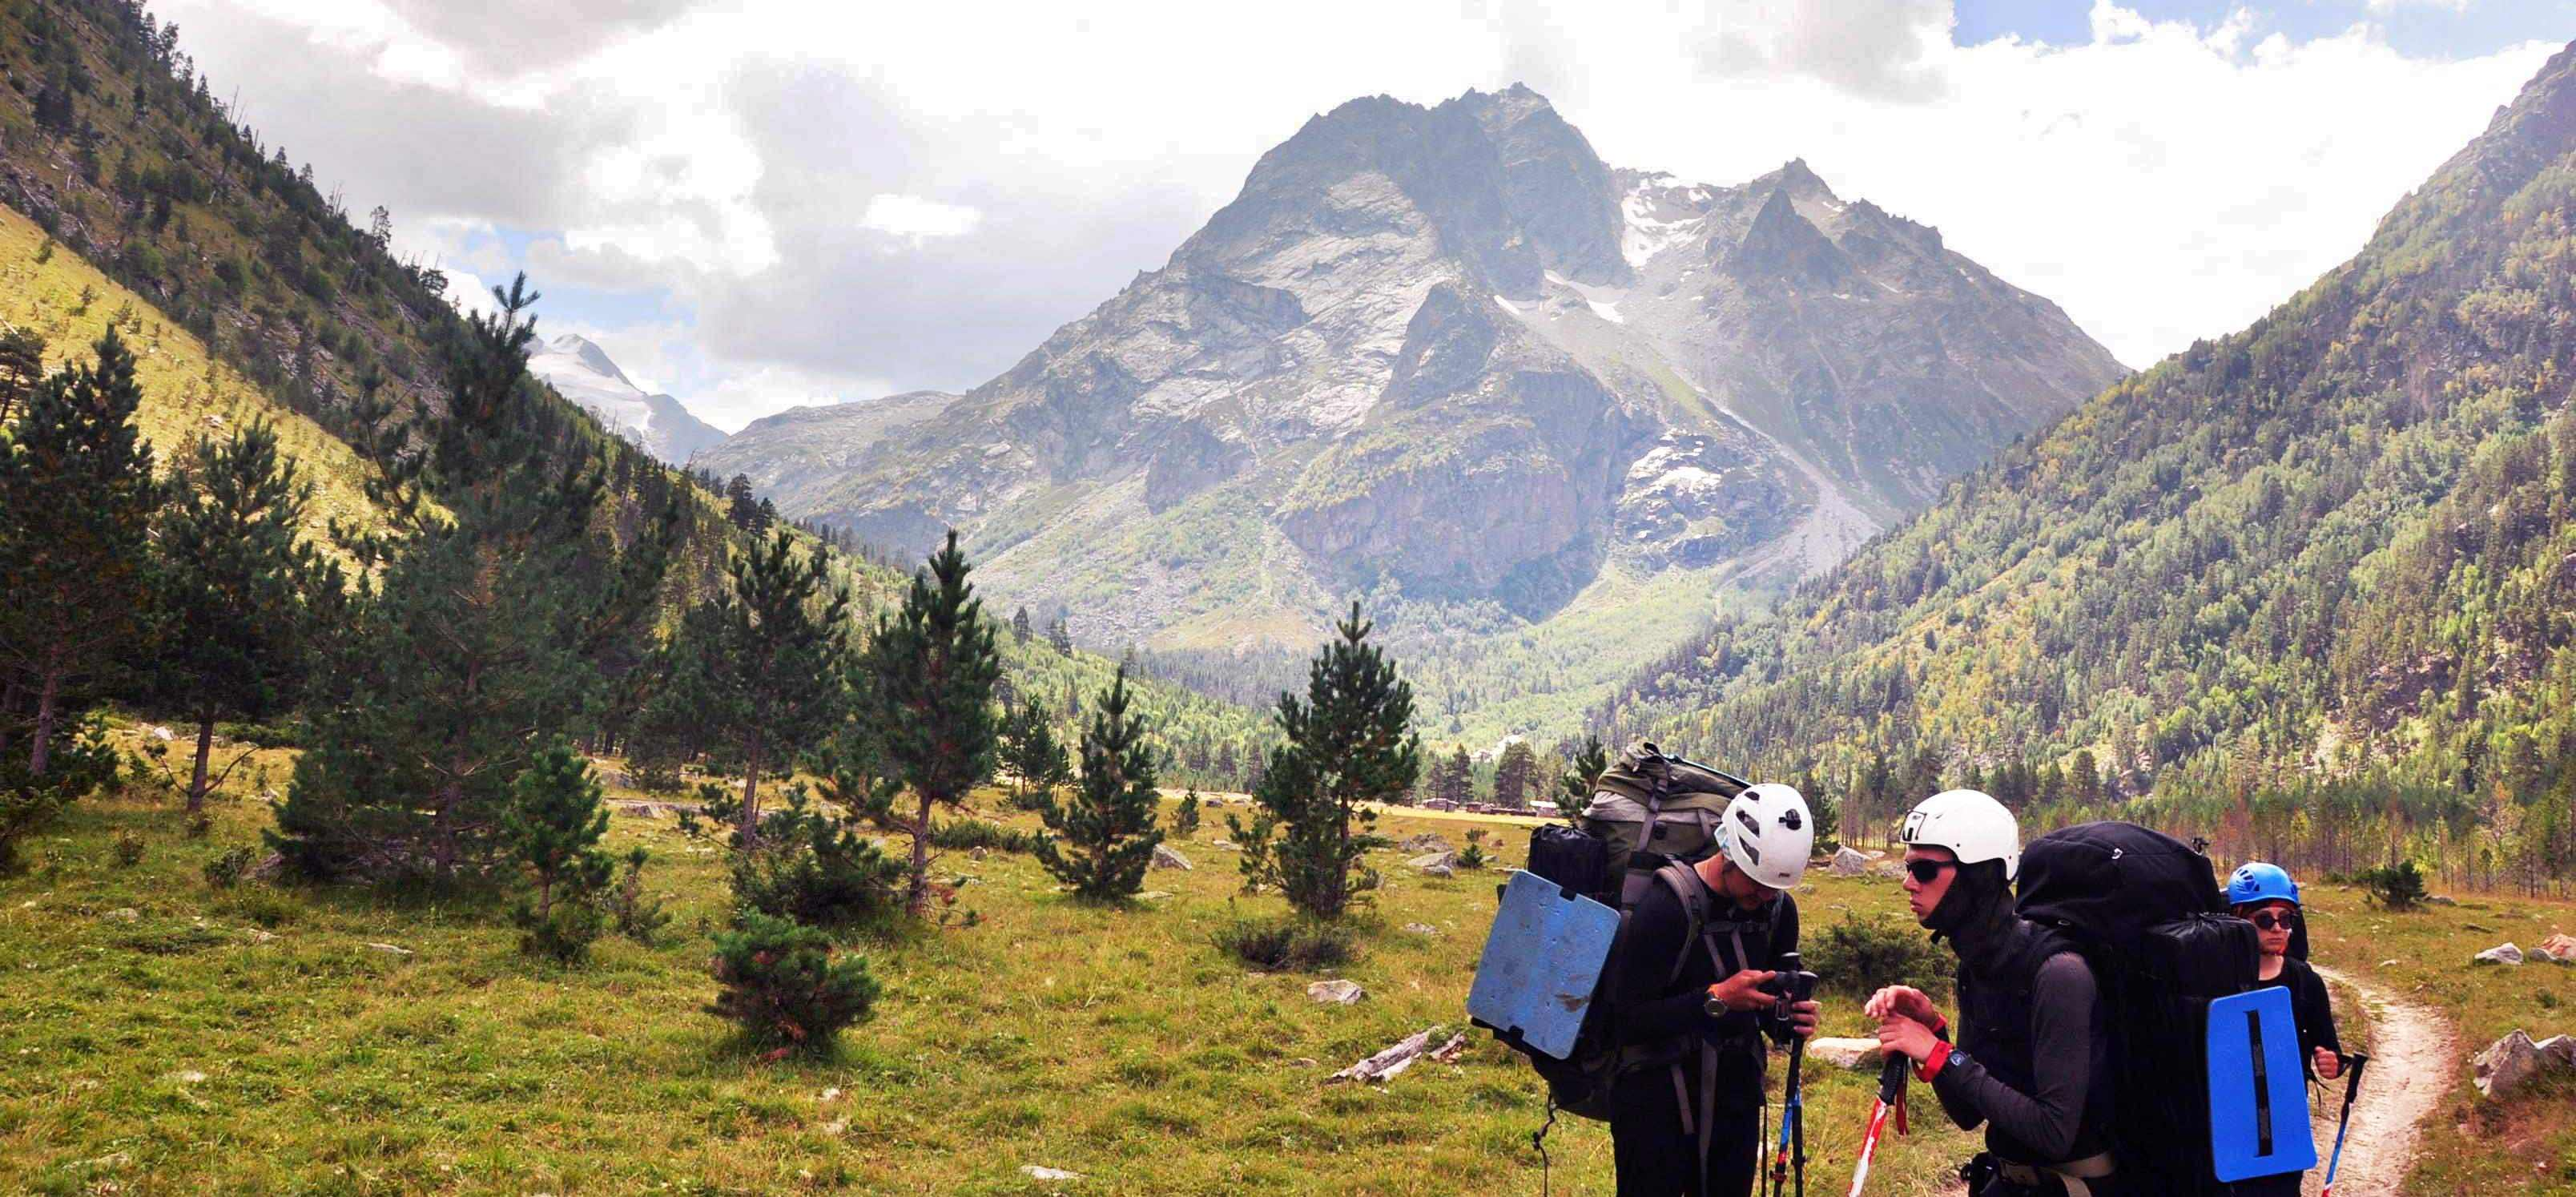
\includegraphics[width=0.7\linewidth]{../pics/DSC_0462 2.JPG}
	\caption{группа в д.р. Кубань}
	\label{fig:DSC_0462 2.JPG}
\end{figure}

Встаем на обед у следующего ручья в (?). Пока мы обедали, подходили конные пограничники, интересовались маршрутом.

\begin{figure}[h!]
	\centering
	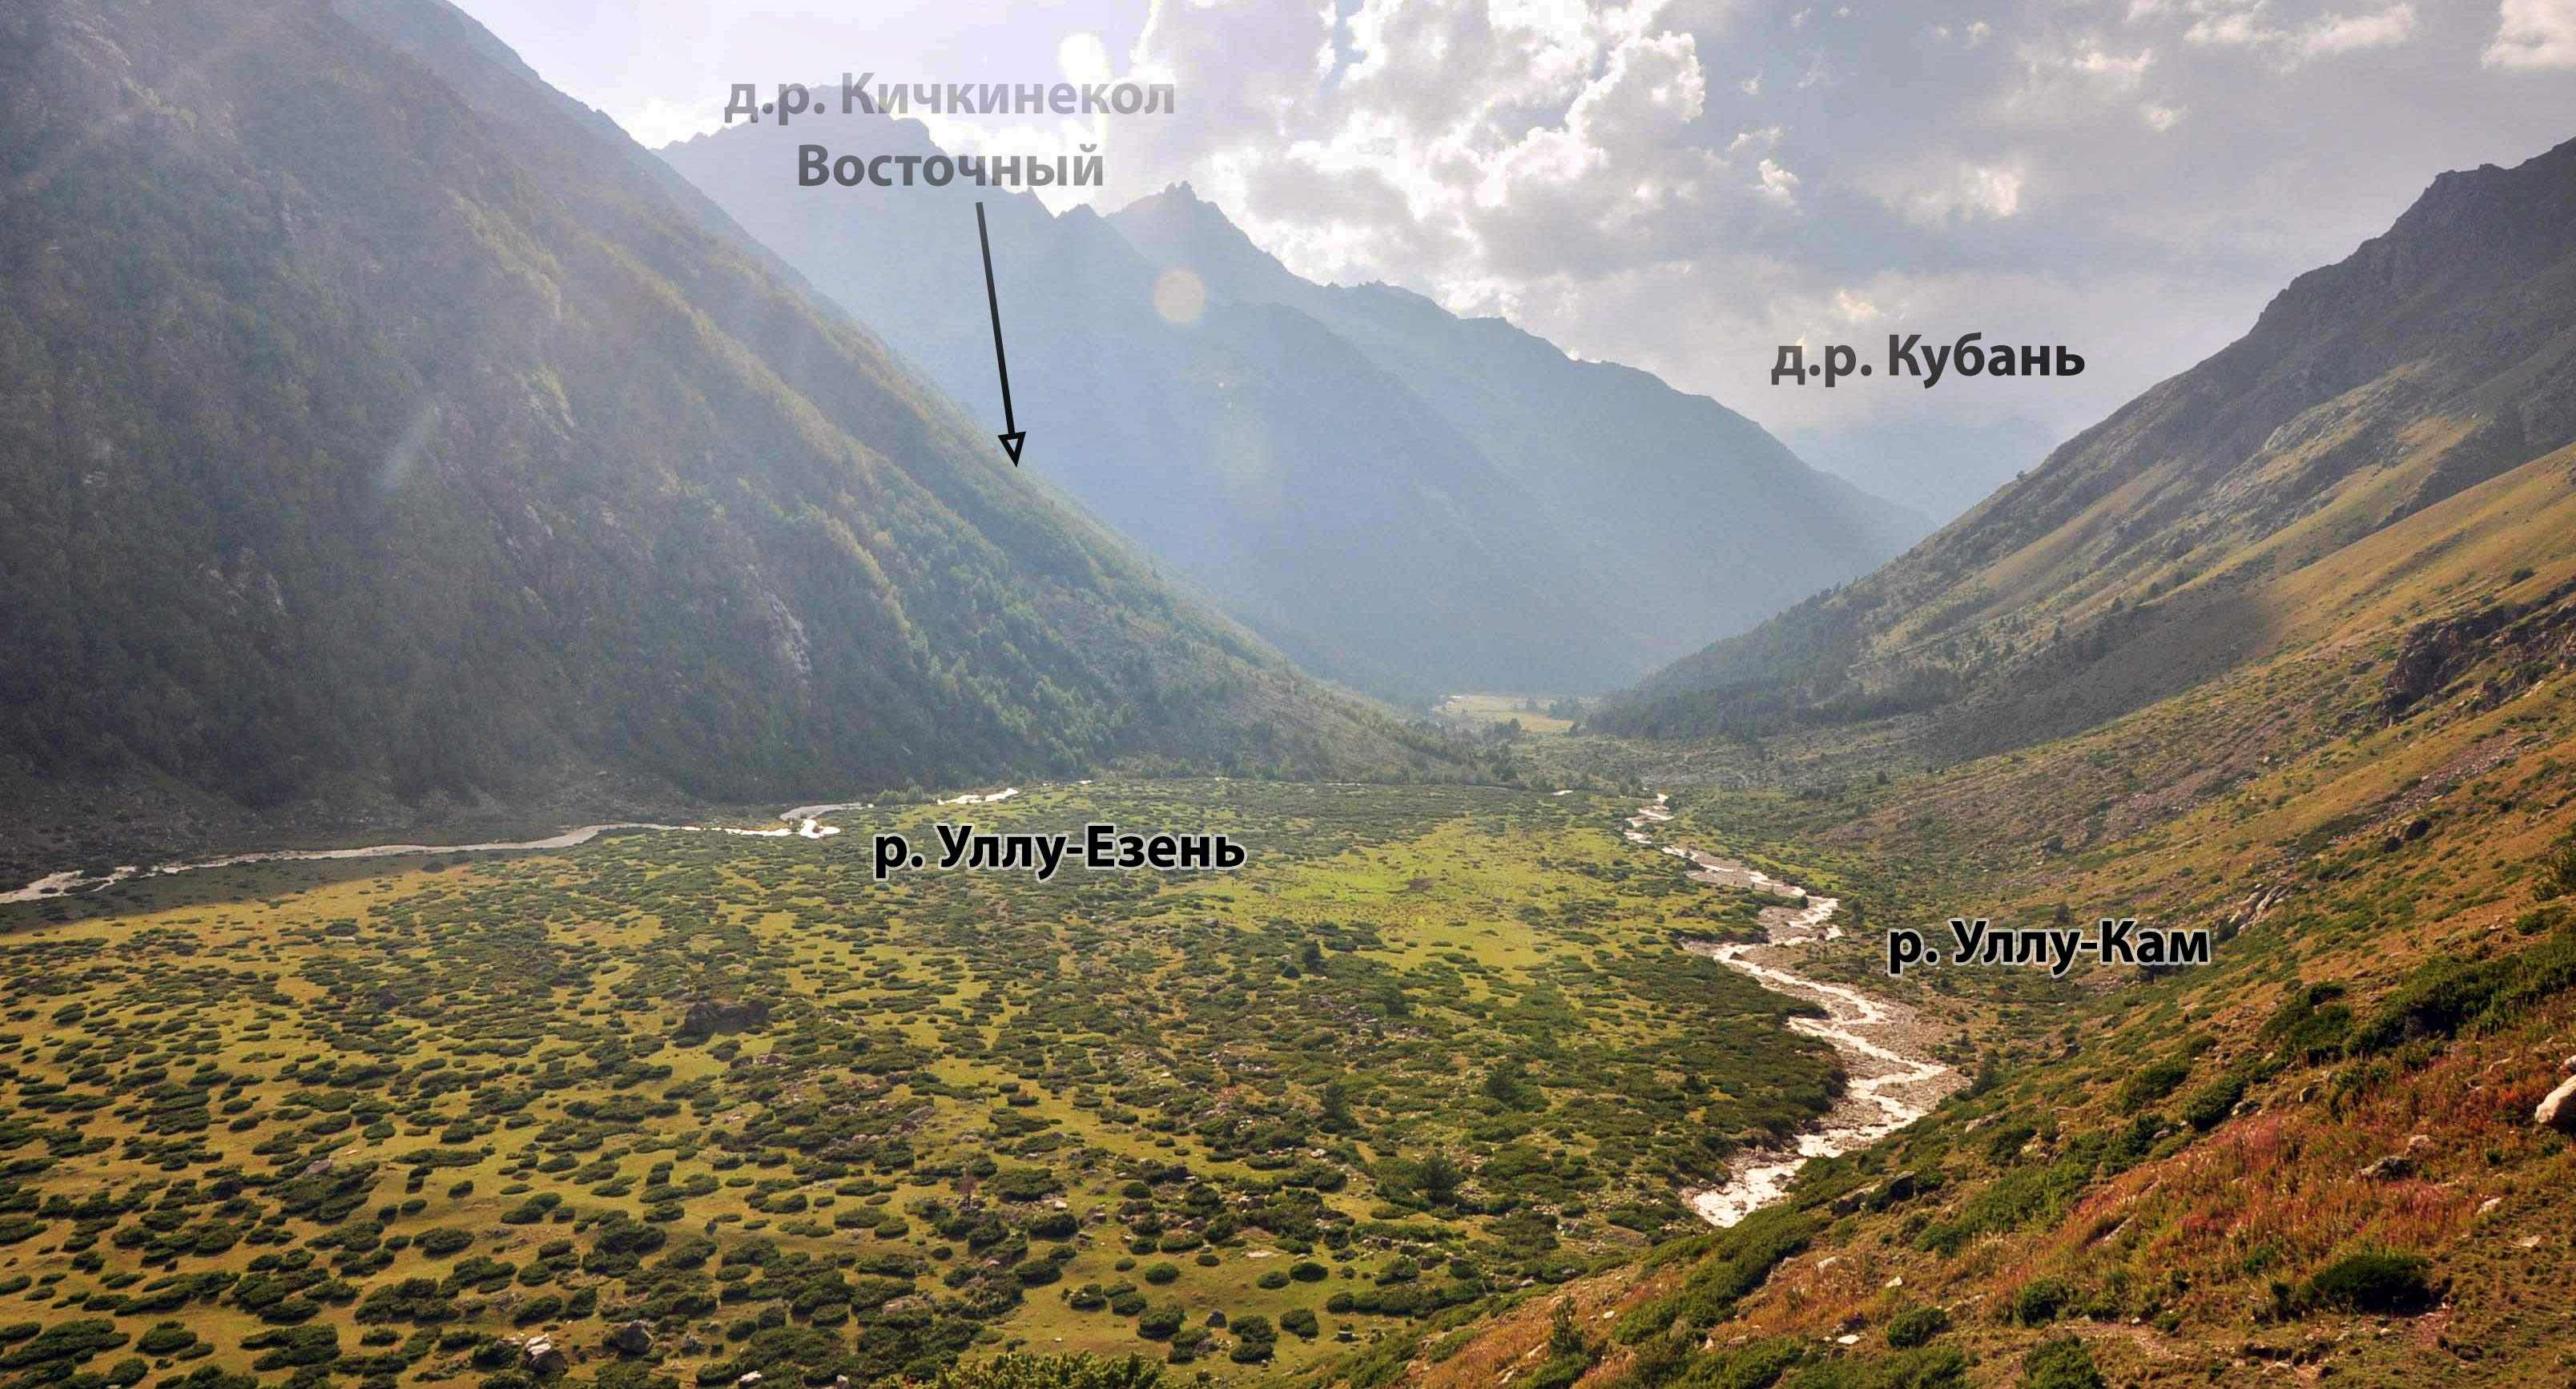
\includegraphics[width=0.7\linewidth]{../pics/DSC_0464 2.JPG}
	\caption{д.р. Кубань, вид с подъема в д.р. Уллу-Кам}
	\label{fig:DSC_0464 2.JPG}
\end{figure}

Продолжаем путь по долине. Постепенно становится облачно.


\begin{figure}[h!]
	\centering
	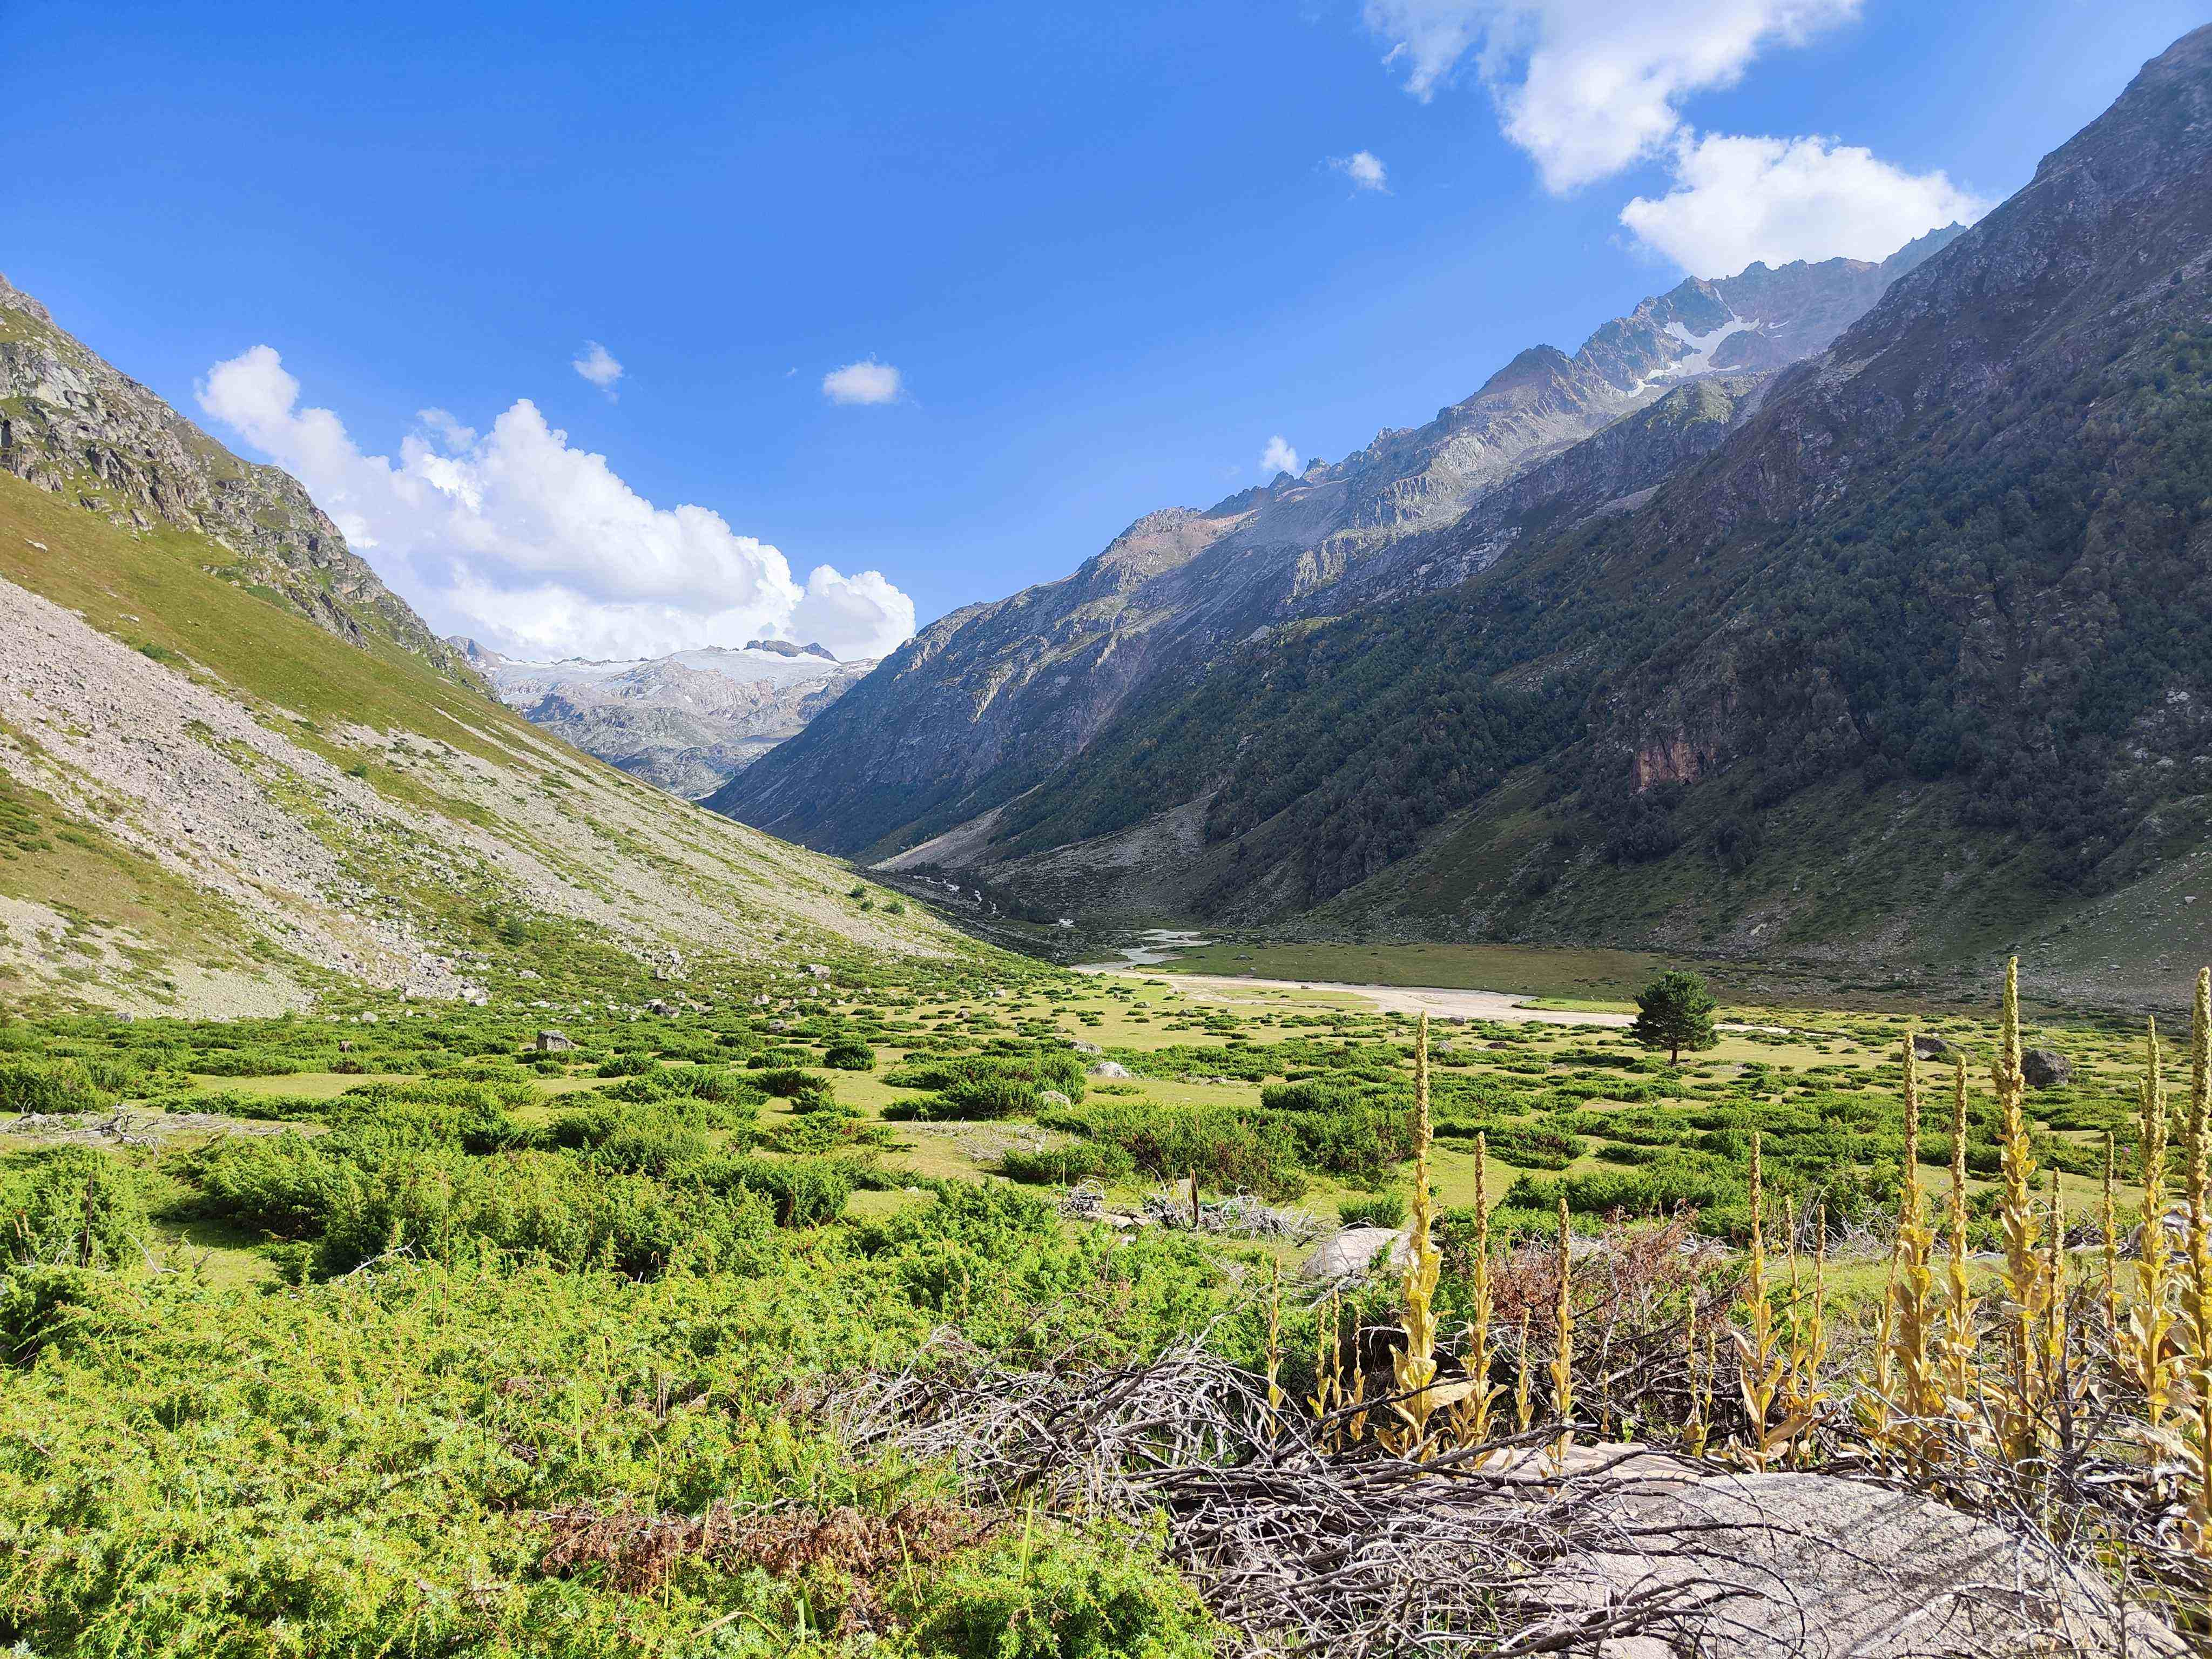
\includegraphics[width=0.7\linewidth]{../pics/IMG_20240829_155915.jpg}
	\caption{долина р. Кубань перед подъемом в долину}
	\label{fig:IMG_20240829_155915.jpg}
\end{figure}

\begin{figure}[h!]
	\centering
	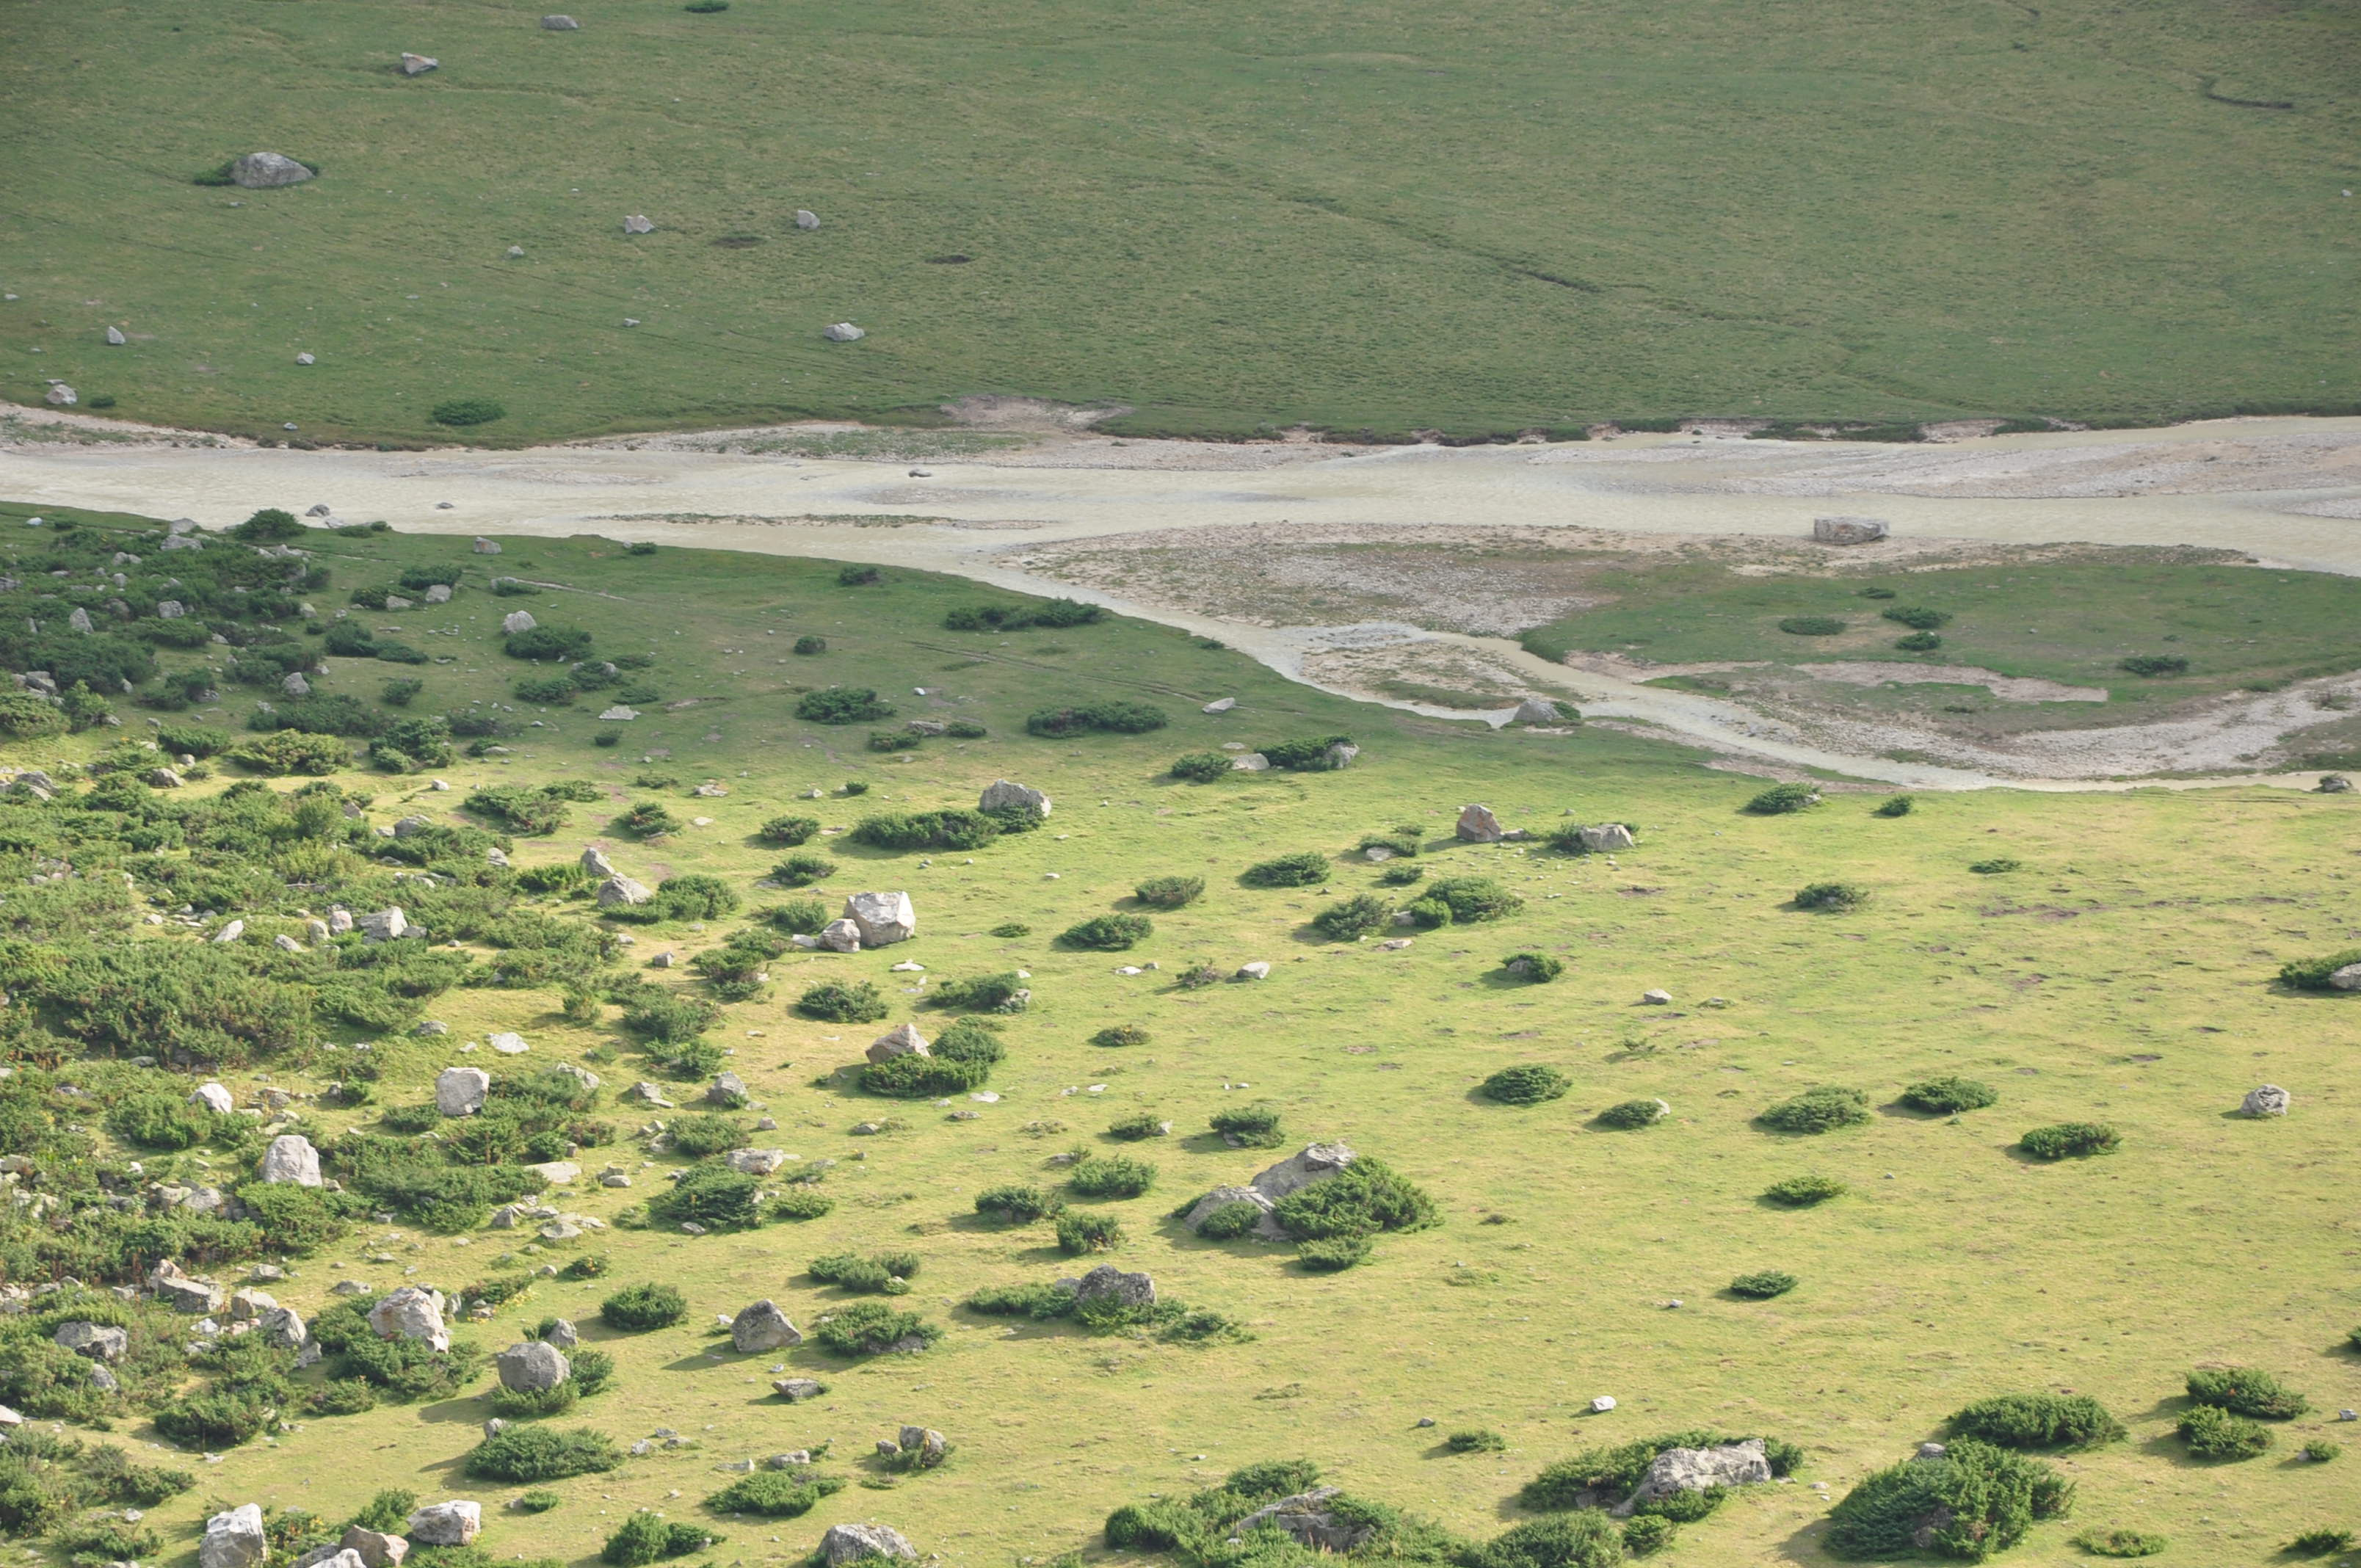
\includegraphics[width=0.7\linewidth]{../pics/DSC_0471 2.JPG}
	\caption{долина, вид с подъема}
	\label{fig:DSC_0471 2.JPG}
\end{figure}

В (?) подходим к подъему в висячую долину, предстоит набрать (?) метров до ночевки. Отдыхаем и начинаем движение.
Идем по размеченной трейловой тропе с палками, временами попадается мелкая сыпуха.

\begin{figure}[h!]
	\centering
	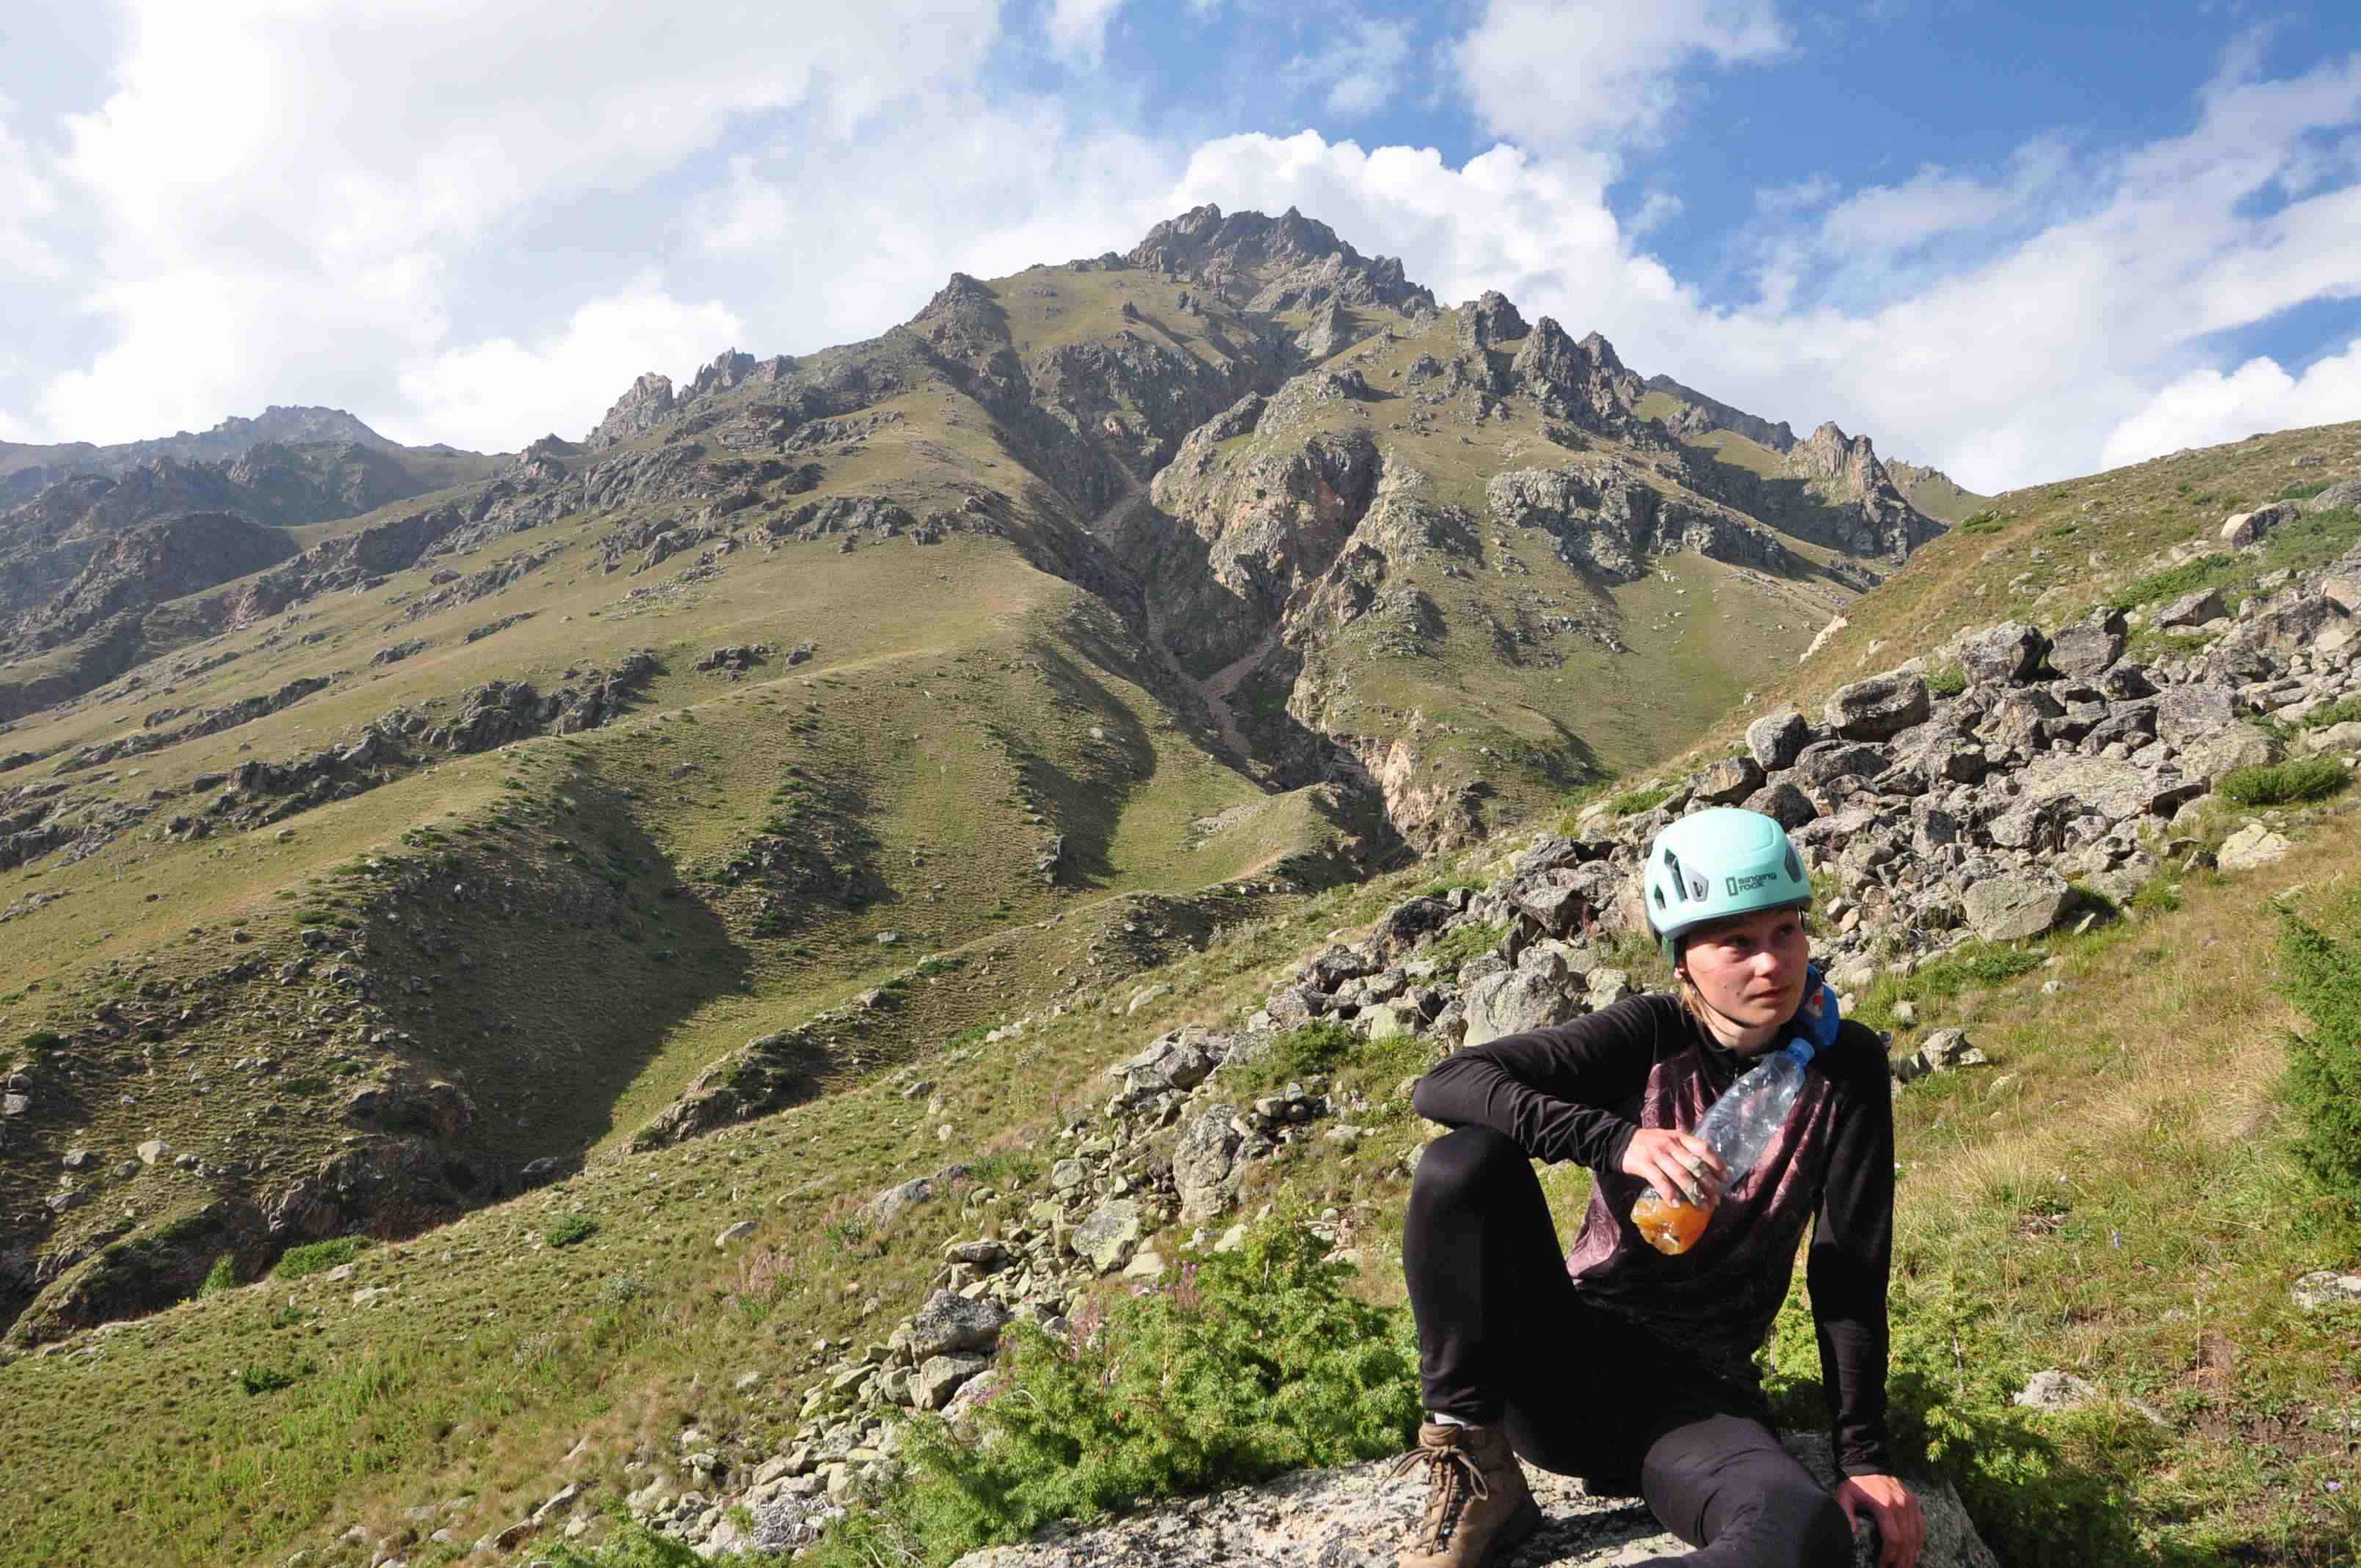
\includegraphics[width=0.7\linewidth]{../pics/DSC_0470 2.JPG}
	\caption{???}
	\label{fig:DSC_0470 2.JPG}
\end{figure}

\begin{figure}[h!]
	\centering
	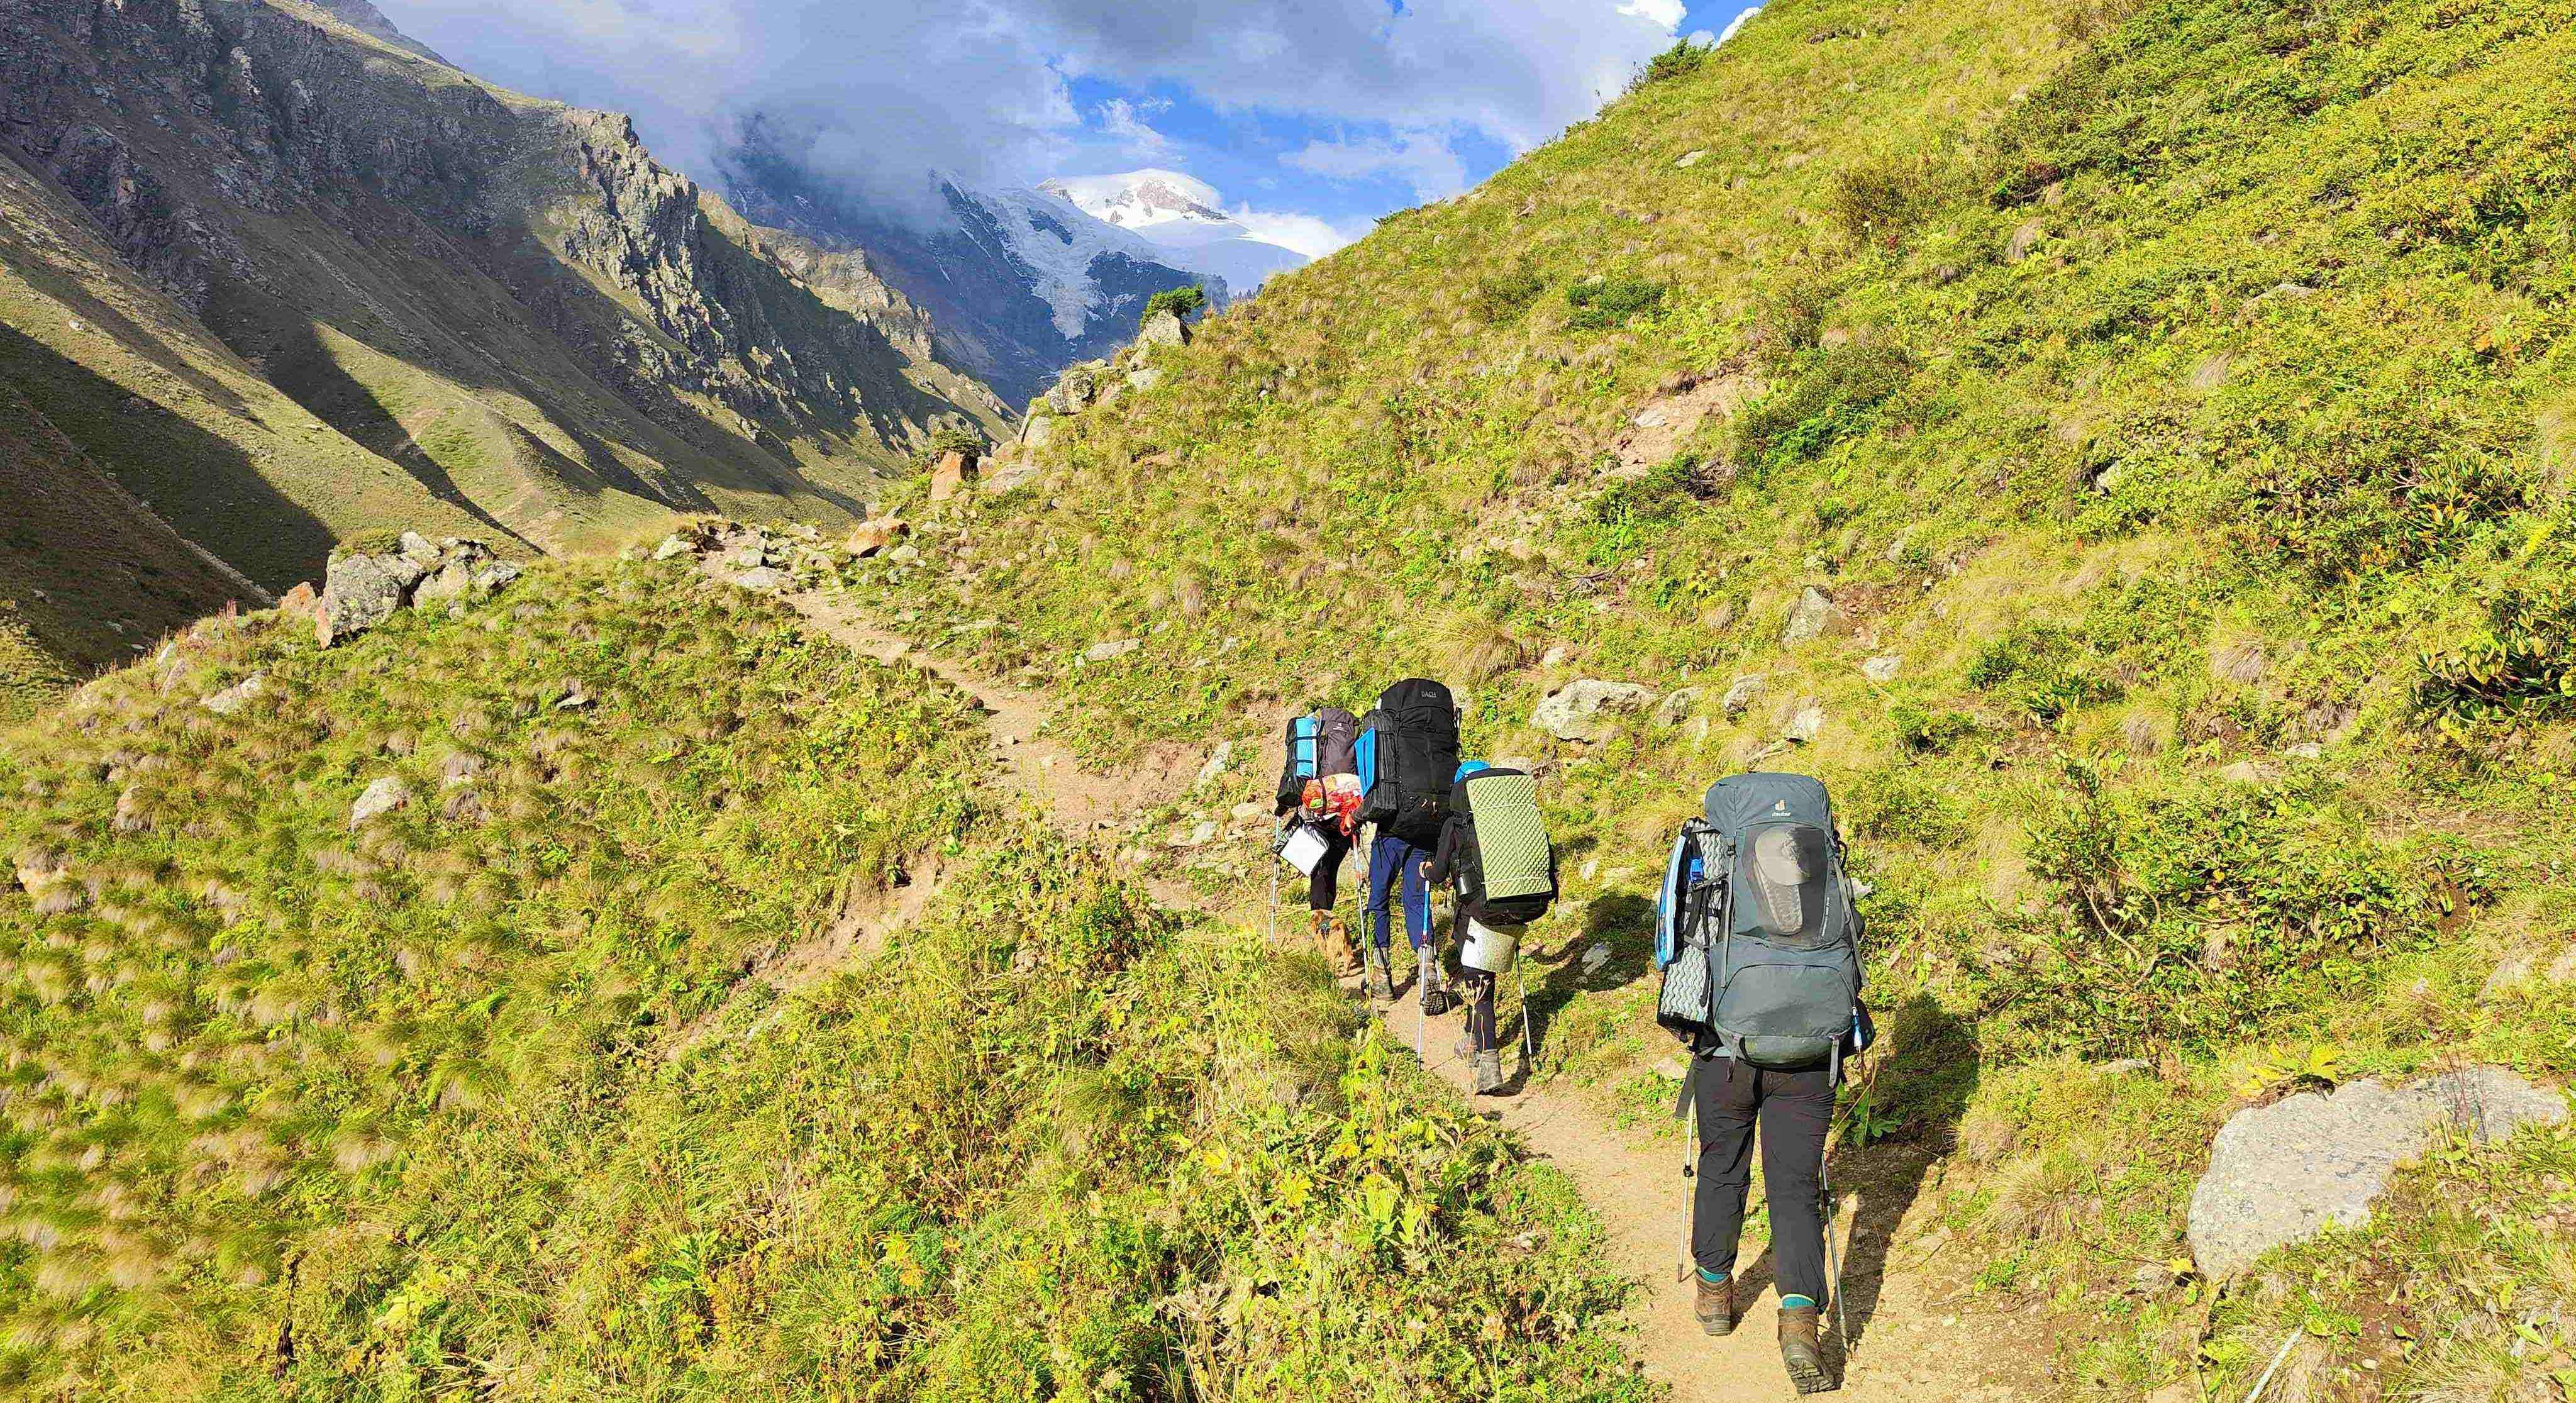
\includegraphics[width=0.7\linewidth]{../pics/IMG_20240829_170756.jpg}
	\caption{Тропа по траверсу}
	\label{fig:IMG_20240829_170756.jpg}
\end{figure}

\begin{figure}[h!]
	\centering
	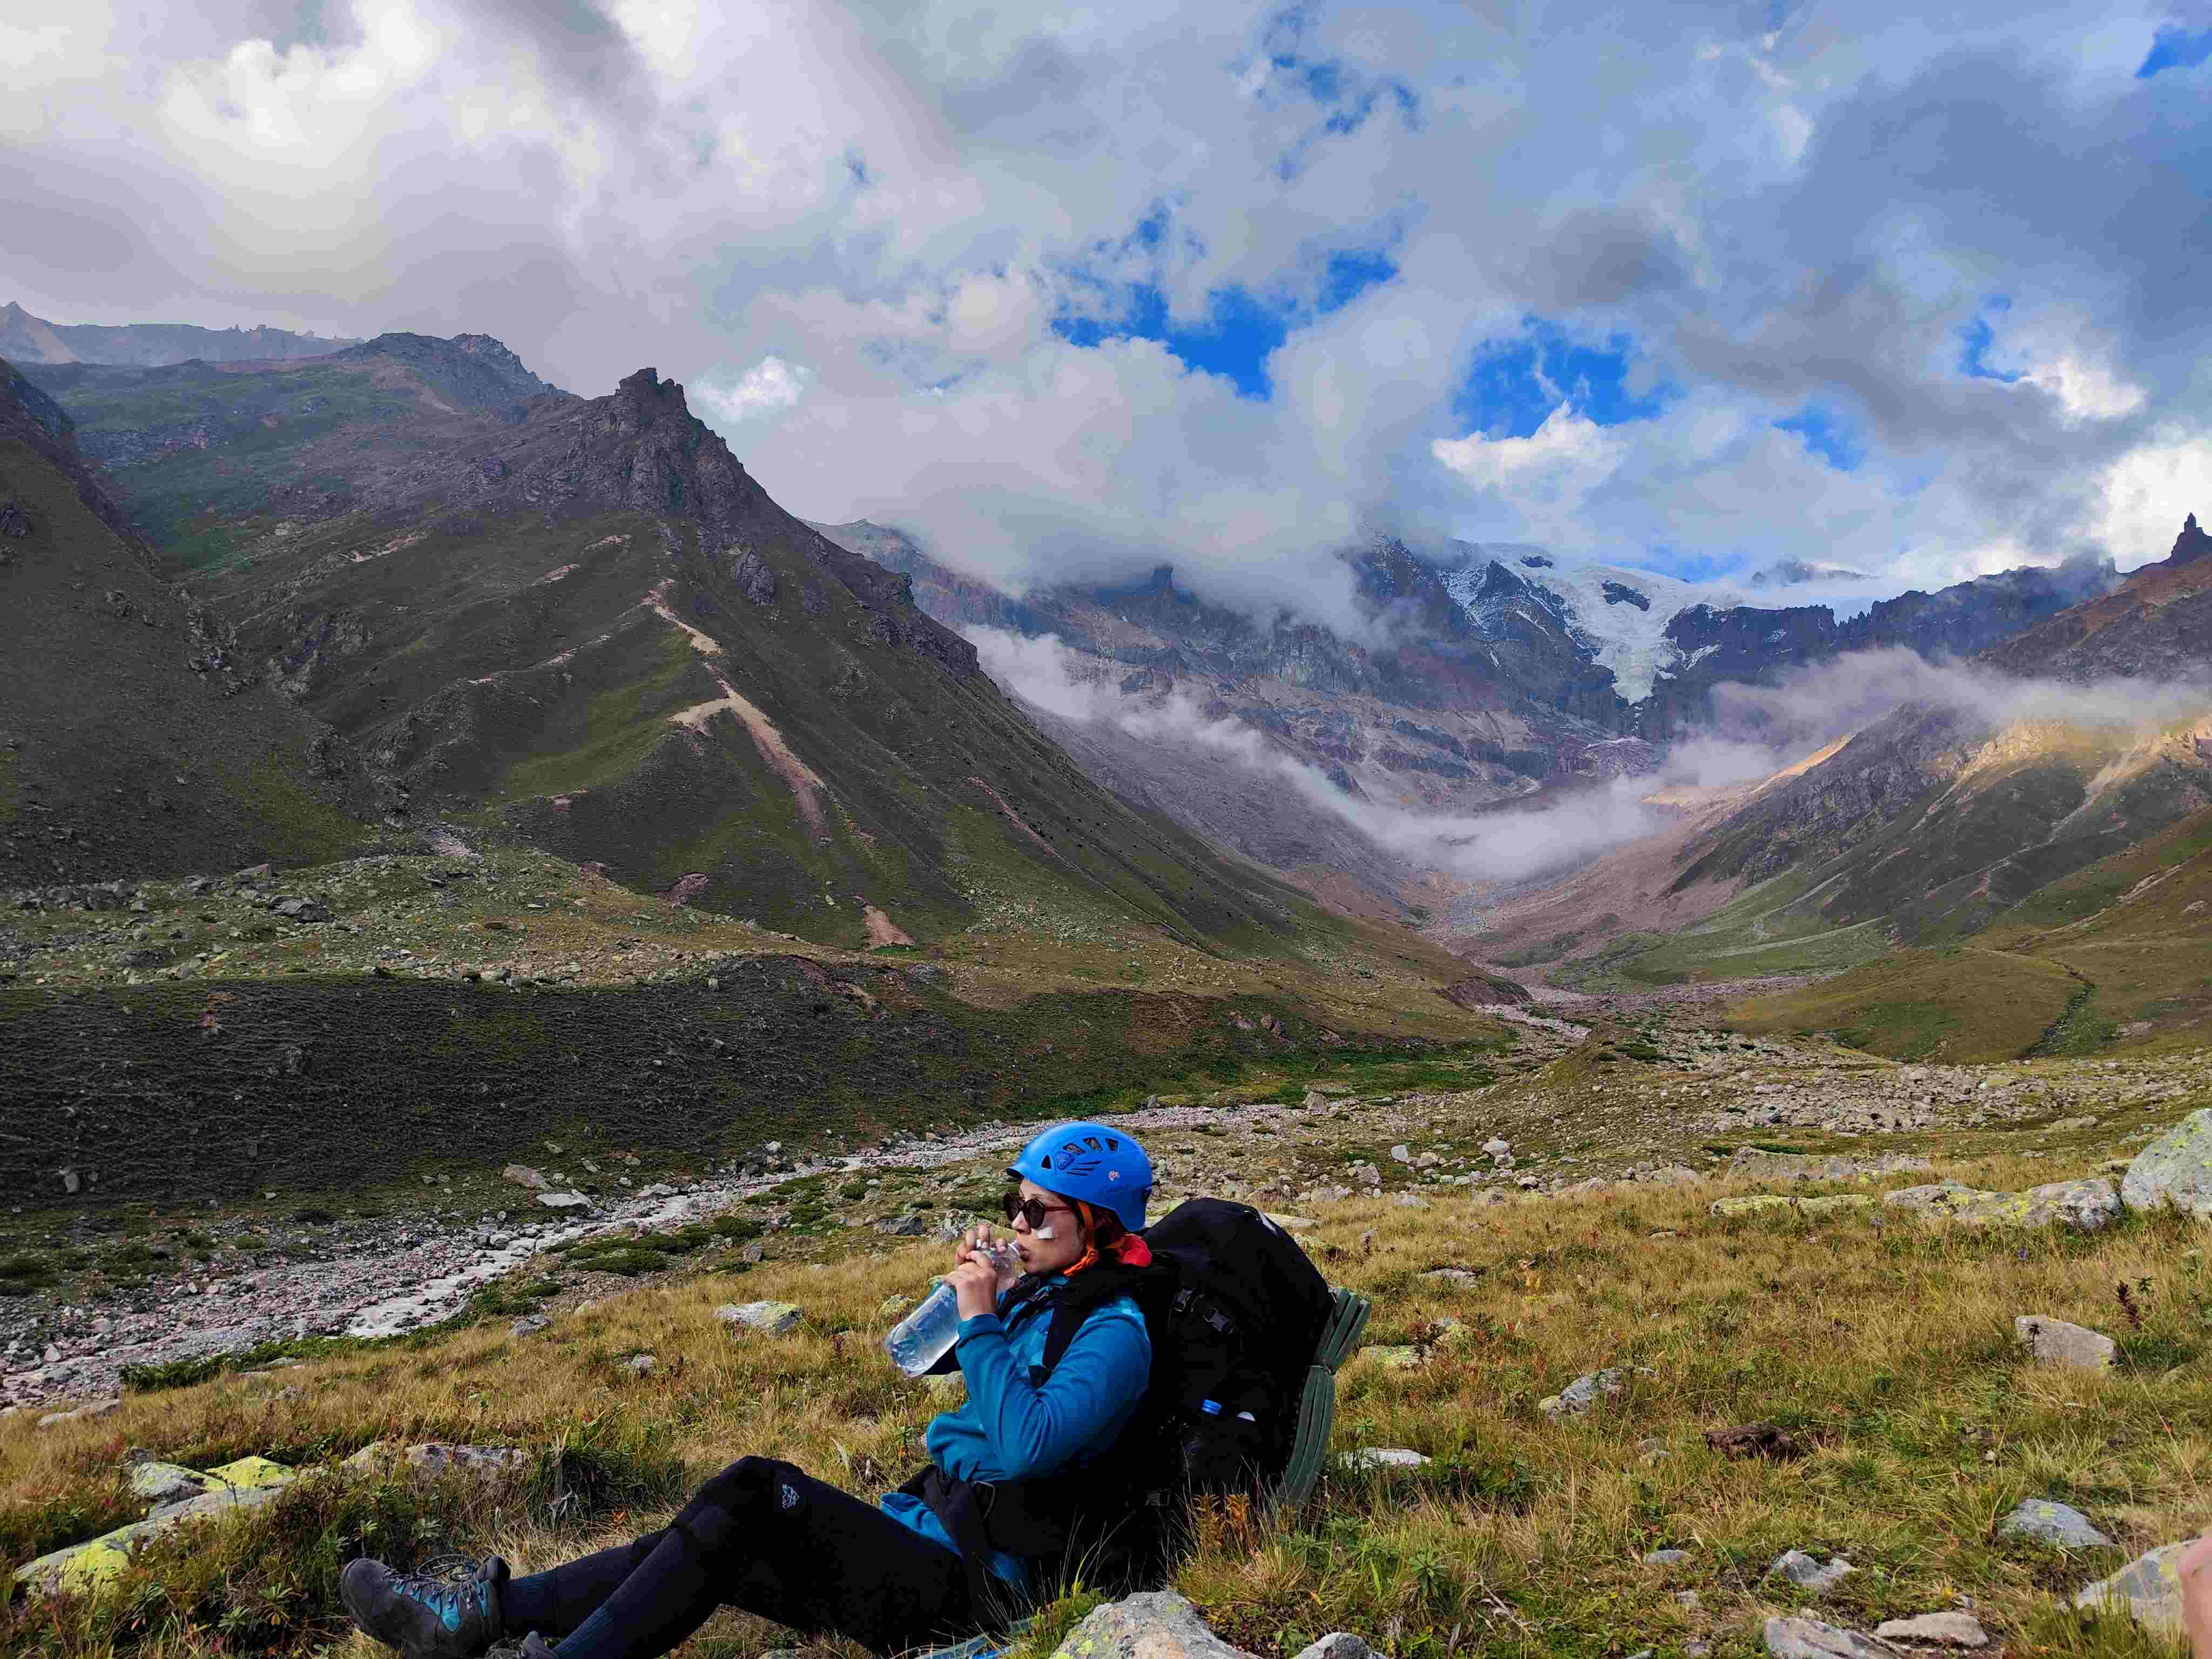
\includegraphics[width=0.7\linewidth]{../pics/IMG_20240829_175721.jpg}
	\caption{???}
	\label{fig:IMG_20240829_175721.jpg}
\end{figure}

\begin{figure}[h!]
	\centering
	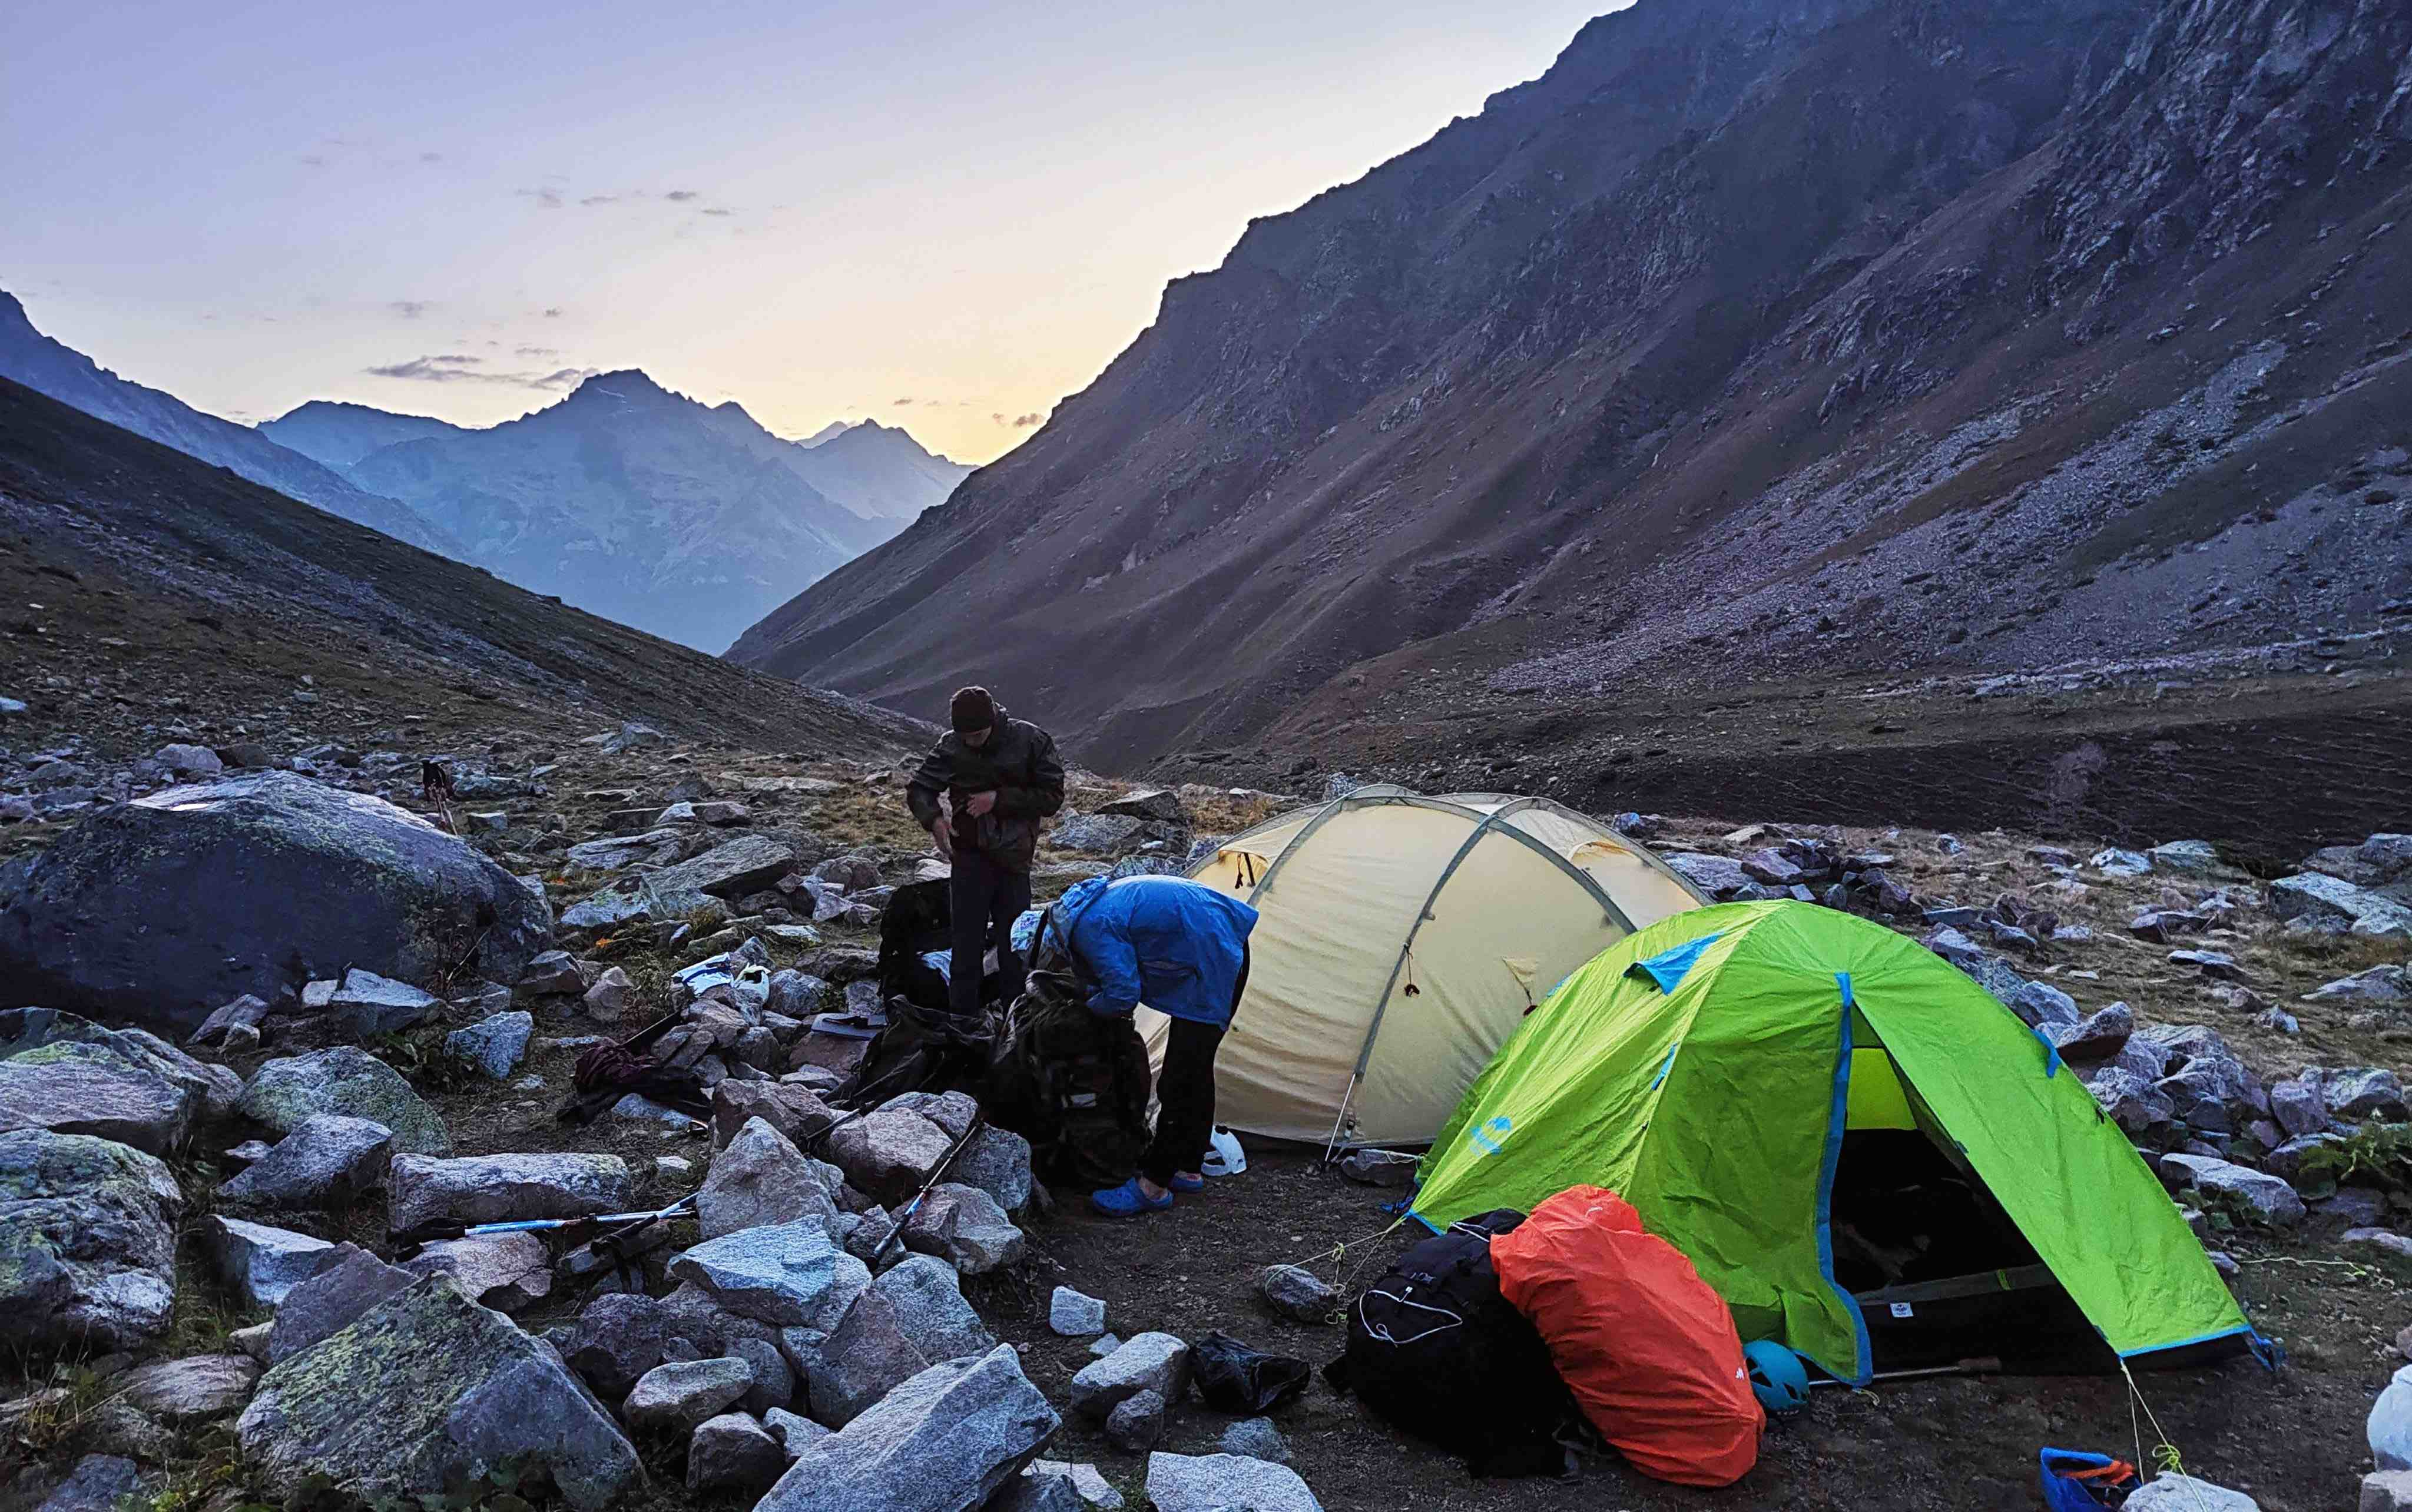
\includegraphics[width=0.7\linewidth]{../pics/IMG_20240829_191225.jpg}
	\caption{разбитый лагерь}
	\label{fig:IMG_20240829_191225.jpg}
\end{figure}

Приходим на место ночевки, есть расчищенные площадки под палатки. Открывается вид на Эльбрус, но быстро затягивается облаками.

\begin{figure}[h!]
	\centering
	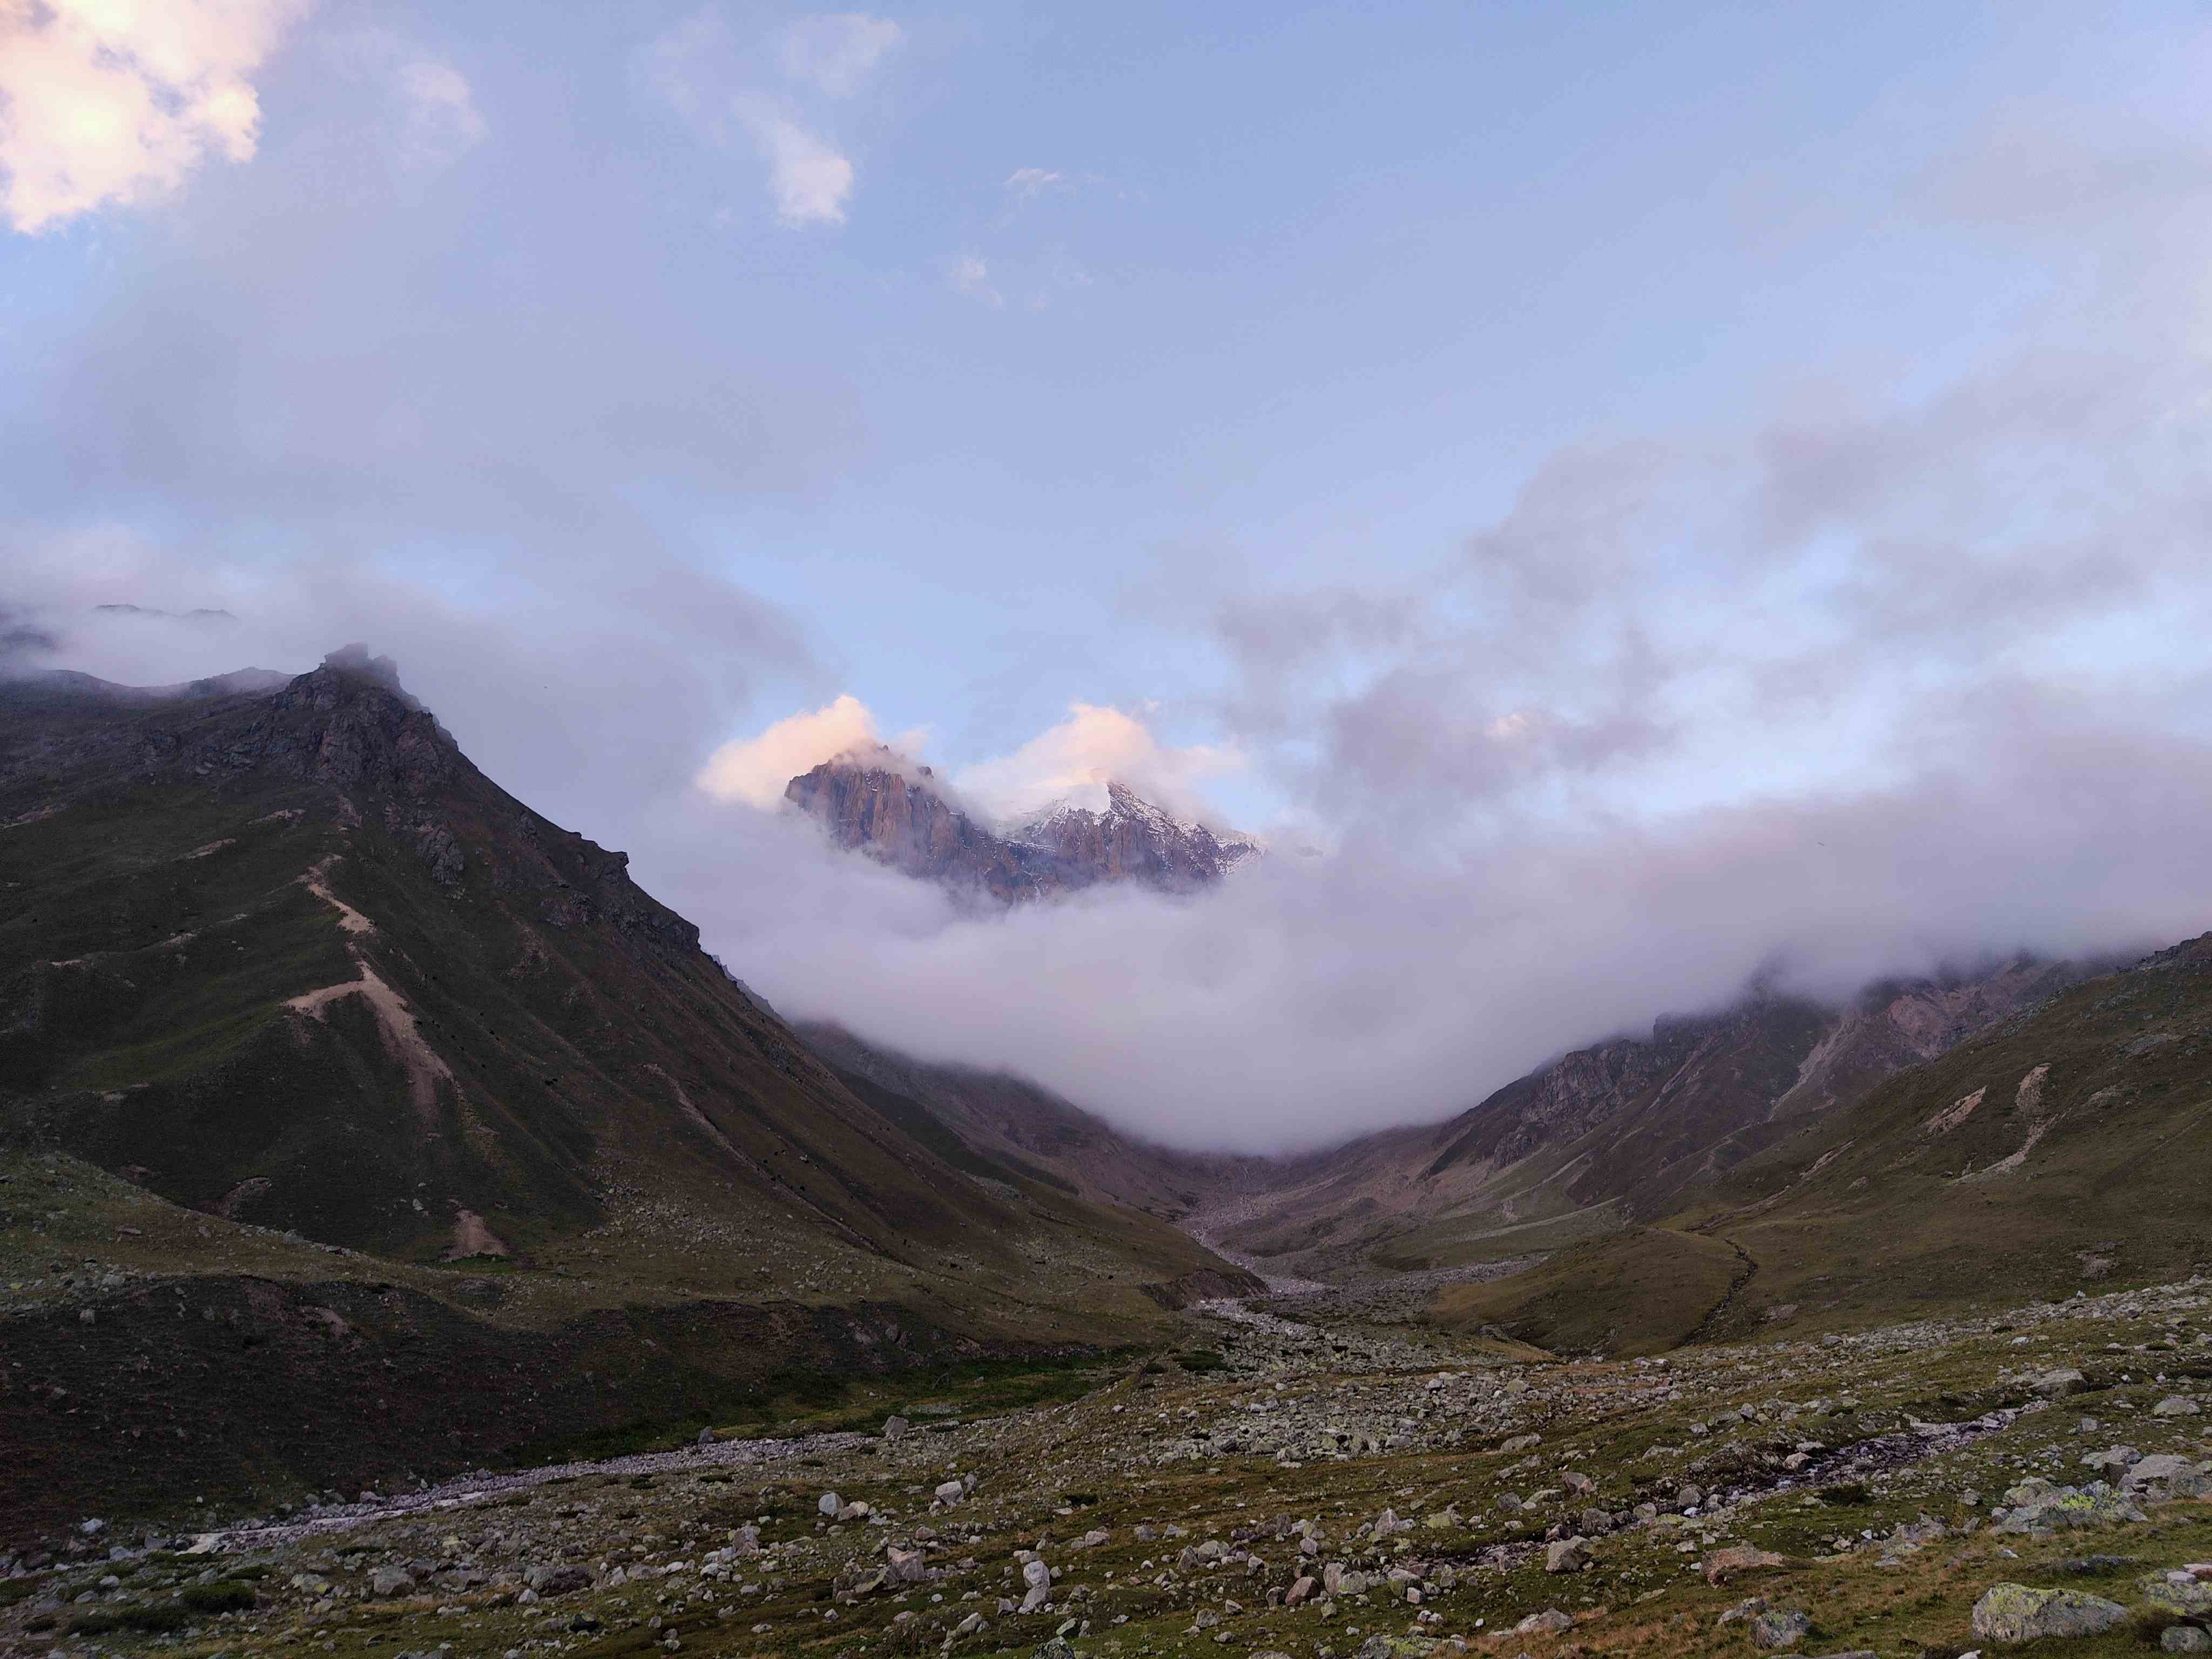
\includegraphics[width=0.7\linewidth]{../pics/IMG_20240829_184033}
	\caption{за облаками - Эльбрус}
	\label{fig:IMG_20240829_184033}
\end{figure}

\newpage